\documentclass{beamer}
\usetheme{Madrid}
\usecolortheme{default}
\usepackage[style=ieee,backend=biber]{biblatex}
\usepackage{graphicx}
% Set language to spanish
\usepackage[spanish]{babel}
\addbibresource{references.bib}

\title{Proyecto de investigación}
\author{Juan Echeagaray}
\institute{Tec de Monterrey}
\date{28 de Agosto del 2023}

\begin{document}
    \frame{\titlepage}

    \begin{frame}
        \frametitle{Agenda}
        \tableofcontents
    \end{frame}

    \section{Introducción}

    \section{Problemática}

        \begin{frame}
            \frametitle{Problemática}
            \begin{block}{Implementación}
                Necesidad de un modelo capaz de estimar la vida útil de un conjunto de máquinas de forma eficiente y confiable
            \end{block}

            \begin{alertblock}{Interpretabilidad}
                Necesidad de un modelo interpretable para entornos críticos donde se requiere explicar el funcionamiento del modelo
            \end{alertblock}

        \end{frame}

    \section{Objetivos}

        \begin{frame}
            \frametitle{Objetivos}
            \begin{itemize}
                \item Metodología de diseño de modelos de predicción de tiempo de vida útil de una flota uniforme de máquinas
                \item Herramientas de interpretación del modelo entrenado
                \item Modelo estable, robusto, reproducible y confiable
            \end{itemize}
        \end{frame}

    \section{Hipótesis}

        \begin{frame}
            \frametitle{Hipótesis}

            \begin{exampleblock}{Hipótesis}
                Utilizando una colección de mediciones de sensores de una flota uniforme de máquinas en conjunto con descriptores ambientales, es posible entrenar un modelo de predicción integrado de tiempo de vida útil que sea estable, robusto, reproducible y confiable.
            \end{exampleblock}
        \end{frame}

    \section{Metodología}

        \begin{frame}
            \frametitle{Metodología}
            \centering
            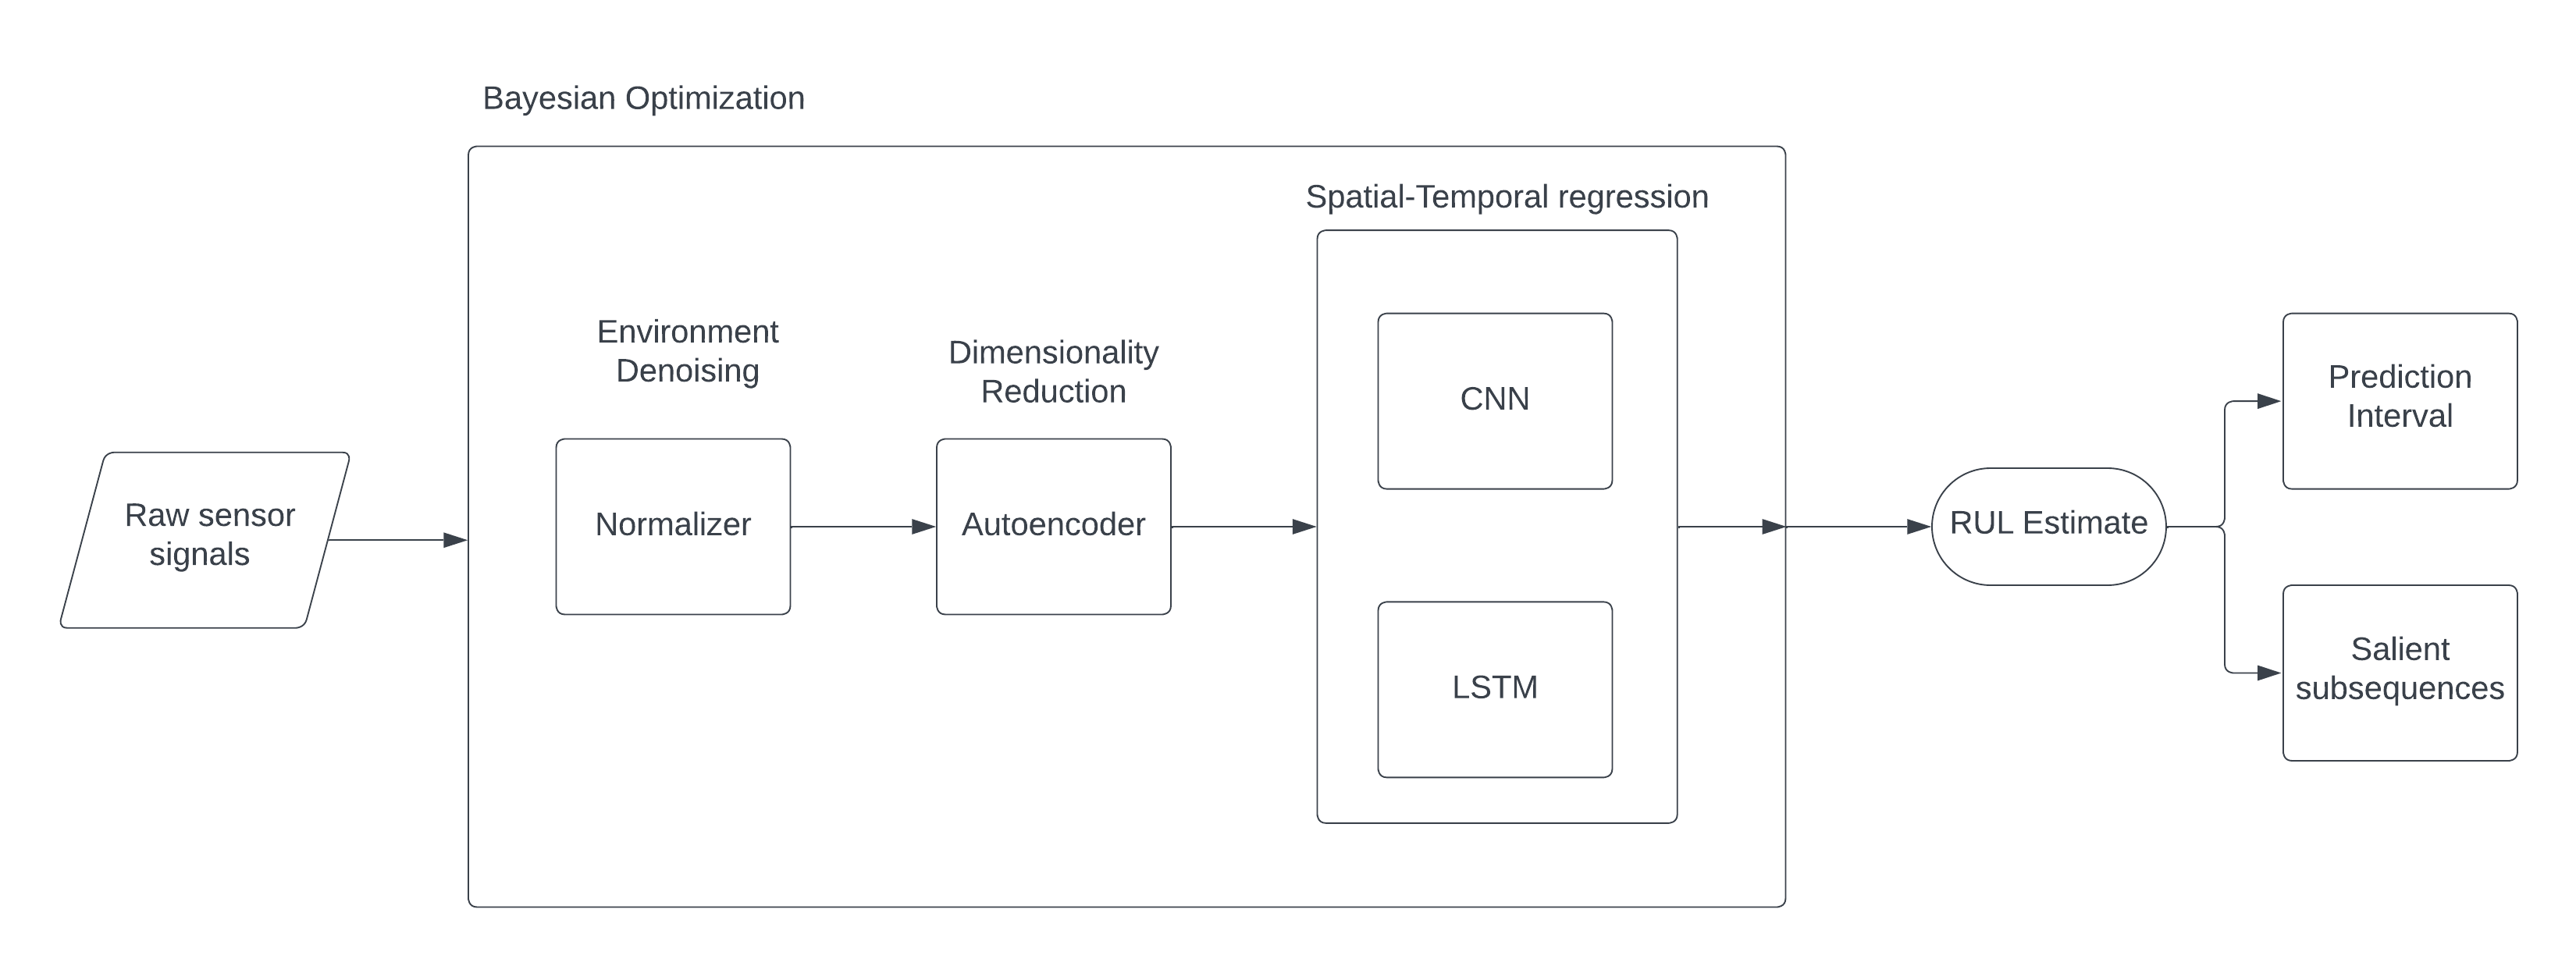
\includegraphics[scale=0.4]{img/pdm-ml-process.png}
        \end{frame}

    \section{Alcance}

        \begin{frame}
            \frametitle{Alcance}
            \begin{itemize}
                \item Predicción de tiempo de vida útil de una flota uniforme de máquinas
                \item Disponibilidad de un conjunto de datos etiquetado con información hasta el punto de falla de las máquinas
            \end{itemize}
        \end{frame}

    \section{Contribuciones}

        \begin{frame}
            \frametitle{Contribuciones}
            \begin{itemize}
                \item Metodología de diseño de modelos de predicción de tiempo de vida útil de una flota uniforme de máquinas
                \item Herramientas de interpretación del modelo entrenado
                \item Librería de Python para la implementación de la metodología
            \end{itemize}
        \end{frame}

\end{document}